% Nature-style figure — pairwise relations grow quadratically with group size
% build: pdflatex fig-pairwise-growth.tex
\documentclass[border=2pt]{standalone}
\usepackage[T1]{fontenc}
\usepackage[scaled=1.0]{helvet}
\renewcommand{\familydefault}{\sfdefault}
\usepackage{amsmath}
\usepackage{sansmath}
\usepackage{anyfontsize}
\usepackage{xcolor}
\usepackage{tikz}
\usepackage{pgfplots}
\pgfplotsset{compat=1.18}
\usetikzlibrary{calc}

\definecolor{ink}{HTML}{1A1A1A}
\definecolor{acc}{HTML}{2F5D8C}
\definecolor{lgt}{HTML}{9FB8CD}
\definecolor{gry}{HTML}{8A8A8A}

\newcommand{\panellabel}[3]{\node[anchor=north west,font=\bfseries\fontsize{8}{9}\selectfont,
  text=ink] at (#1,#2) {#3};}

% \cgraph{center x}{center y}{N}{radius}
\newcommand{\cgraph}[4]{%
  \foreach \i in {1,...,#3}{%
    \foreach \j in {1,...,#3}{%
      \ifnum\i<\j
        \draw[lgt,line width=0.16pt]
          ({#1+#4*cos(90+(\i-1)*360/#3)},{#2+#4*sin(90+(\i-1)*360/#3)}) --
          ({#1+#4*cos(90+(\j-1)*360/#3)},{#2+#4*sin(90+(\j-1)*360/#3)});
      \fi}}%
  \foreach \i in {1,...,#3}{%
    \filldraw[fill=white,draw=acc,line width=0.28pt]
      ({#1+#4*cos(90+(\i-1)*360/#3)},{#2+#4*sin(90+(\i-1)*360/#3)}) circle (0.55);}%
}

\begin{document}
\sansmath\fontsize{7}{8.4}\selectfont
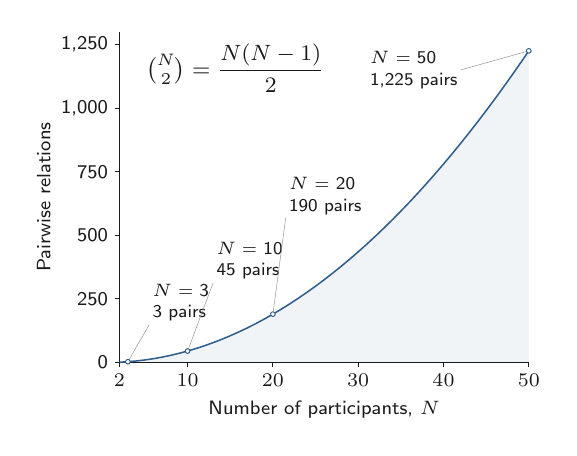
\begin{tikzpicture}[font=\fontsize{7}{8.4}\selectfont,text=ink]
\begin{axis}[
  width=52mm, height=42mm, scale only axis,
  axis lines=left,
  axis line style={line width=0.3pt, ink, -},
  tick align=outside,
  xtick style={line width=0.3pt, ink}, ytick style={line width=0.3pt, ink},
  major tick length=1.6pt,
  xmin=2, xmax=50, ymin=0, ymax=1300,
  xtick={2,10,20,30,40,50},
  ytick={0,250,500,750,1000,1250},
  yticklabels={0,250,500,750,{1,000},{1,250}},
  xlabel={Number of participants, $N$},
  ylabel={Pairwise relations},
  xlabel style={font=\fontsize{7}{8.4}\selectfont, yshift=1.5pt},
  ylabel style={font=\fontsize{7}{8.4}\selectfont, yshift=-3pt},
  tick label style={font=\fontsize{7}{8.4}\selectfont},
  x tick label style={yshift=1pt}, y tick label style={xshift=1pt},
  clip=false,
]

\addplot[draw=none, fill=acc, fill opacity=0.07, domain=2:50, samples=49]
  {x*(x-1)/2} \closedcycle;
\addplot[acc, line width=0.55pt, domain=2:50, samples=49] {x*(x-1)/2};
\addplot[only marks, mark=*, mark size=0.85pt,
  mark options={fill=white, draw=acc, line width=0.35pt}]
  coordinates {(3,3) (10,45) (20,190) (50,1225)};

\node[anchor=north west, font=\fontsize{8}{9}\selectfont]
  at (axis cs:4.0,1290) {$\binom{N}{2}=\dfrac{N(N-1)}{2}$};

\newcommand{\ann}[5]{%
  \node[anchor=west, align=left, font=\fontsize{6.5}{7.8}\selectfont, inner sep=1pt]
    (annnode) at (axis cs:#3,#4) {$N$ = #1\\ #2\ pairs};
  \draw[gry, line width=0.16pt] (annnode.#5) -- (axis cs:#1,{#1*(#1-1)/2});
}
\ann{3}{3}{5.5}{235}{south west}
\ann{10}{45}{13}{400}{south west}
\ann{20}{190}{21.5}{655}{south west}
\ann{50}{1{,}225}{31}{1150}{east}

\end{axis}
\end{tikzpicture}
\end{document}
